\documentclass[12pt,a4paper]{ctexart}
\usepackage[margin=2.2cm]{geometry}
\usepackage{graphicx}
\usepackage{booktabs}
\usepackage{amsmath}
\usepackage{float}
\usepackage{hyperref}
\usepackage{xcolor}
\usepackage{listings}

\lstset{
  language=Python,
  basicstyle=\ttfamily\small,
  keywordstyle=\color{blue!70!black},
  commentstyle=\color{green!40!black},
  stringstyle=\color{orange!60!black},
  showstringspaces=false,
  breaklines=true,
  frame=single,
  tabsize=4
}

\title{聚类实验报告：KMeans、层次聚类与DBSCAN对比}
\author{姓名：\underline{\hspace{3cm}} \quad 学号：\underline{\hspace{3cm}}}
\date{\today}

\begin{document}
\maketitle

\section{实验目的}
本实验围绕无监督聚类展开，目标如下：
\begin{itemize}
  \item 在二维点数据、时序数据和 UCI 数据集上完成聚类实验，并比较不同算法的适应性。
  \item 手工实现 KMeans 与 single-link 层次聚类（SLINK），并与 sklearn 实现进行对照。
  \item 通过聚类图、ARI、NMI、运行时间和内存占用分析参数对结果的影响。
\end{itemize}

\section{实验过程}
\subsection{实验环境}
\begin{itemize}
  \item 操作系统：Linux
  \item 编程语言：Python 3
  \item 主要工具：NumPy、Pandas、Matplotlib、scikit-learn
  \item 报告目录结构参考了 \texttt{Machine-Learning/lab-cnn-rnn/lab-report}
\end{itemize}

\subsection{数据集与预处理}
\begin{itemize}
  \item 二维点数据：\texttt{dots/clusterData*.dat}，每行包含一个二维坐标点，主要用于观察不同聚类算法对几何形状的划分效果。
  \item 时序数据：\texttt{timeSeries/Plane\\_TRAIN.txt}，首列为标签，其余为时序值。实验中对数值部分做标准化，并进一步提取统计特征。
  \item UCI 数据：\texttt{wine+quality/winequality-red.csv} 与 \texttt{winequality-white.csv}，将两份数据合并后以质量标签作为参考类别。
\end{itemize}

\subsection{在原有文件基础上的改动}
原始工程中，\texttt{kmeans.py}、\texttt{linkage.py} 和 \texttt{dbscan.py} 主要是对 sklearn 的简单封装，\texttt{clustering.py} 负责读入数据并调用模型。为了满足实验要求，我在原结构上做了以下补充：
\begin{itemize}
  \item 新增 \texttt{features.py}，为点数据和时序数据提供统一的特征处理入口。
  \item 将 \texttt{kmeans.py} 改为支持手写 KMeans 与 sklearn 双版本对照。
  \item 将 \texttt{linkage.py} 改为支持手写 SLINK（single-link）与 sklearn 双版本对照。
  \item 扩展 \texttt{clustering.py}，加入 UCI 数据读取、结果评估、时间/内存统计、参数扫描和统一输出目录 \texttt{results/}。
  \item 将实验图片统一写入 \texttt{lab-report/images}，报告文件独立放在 \texttt{lab-report/report.tex}，与参考项目的文件管理方式保持一致。
\end{itemize}

\subsection{实现步骤}
\begin{enumerate}
  \item 读取不同类型的数据集并完成归一化或特征提取。
  \item 调用 KMeans、single-link 层次聚类和 DBSCAN 进行聚类，并支持手写实现与 sklearn 实现对照。
  \item 使用 ARI、NMI、运行时间、峰值内存和聚类散点图对结果进行评估与分析。
\end{enumerate}

\section{实验内容}
\subsection{任务一：KMeans 与 single-link 层次聚类对照}
KMeans 通过迭代更新簇中心和样本归属来最小化簇内平方误差，适合紧凑、近似球形的数据簇。single-link 层次聚类则按照最近邻距离逐步合并簇，更容易形成链式结构。

主要参数：
\begin{itemize}
  \item KMeans 的簇数设为 5，初始化方式为 random。
  \item 层次聚类使用 single linkage，并同样设置簇数为 5。
  \item 为了比较实现差异，手写版和 sklearn 版都执行一次。
\end{itemize}

实现要点：
\begin{itemize}
  \item KMeans 手写版直接使用 NumPy 计算样本到中心的距离、更新中心并判断收敛。
  \item SLINK 手写版通过最近邻链接关系构造单链层次结构，再切分出指定簇数。
\end{itemize}

\subsection{任务二：DBSCAN 与参数敏感性}
DBSCAN 是基于密度的聚类方法，不需要预先指定簇数，可以检测任意形状簇并将低密度区域判为噪声。其核心参数是 \texttt{eps} 和 \texttt{min\_samples}，对尺度非常敏感。

\subsection{任务三：不同数据集上的聚类表现}
在时序数据和 UCI 数据集上，使用 ARI 和 NMI 衡量聚类标签与真实标签的一致性；在二维点数据上主要观察聚类图的几何划分效果。

\section{实验结果}
\subsection{任务一结果：二维点数据的聚类图}
二维点数据对应的图像如下，结果都保存到 \texttt{results/} 下，并在图例中标明算法、实现方式和参数。

\begin{figure}[H]
\centering
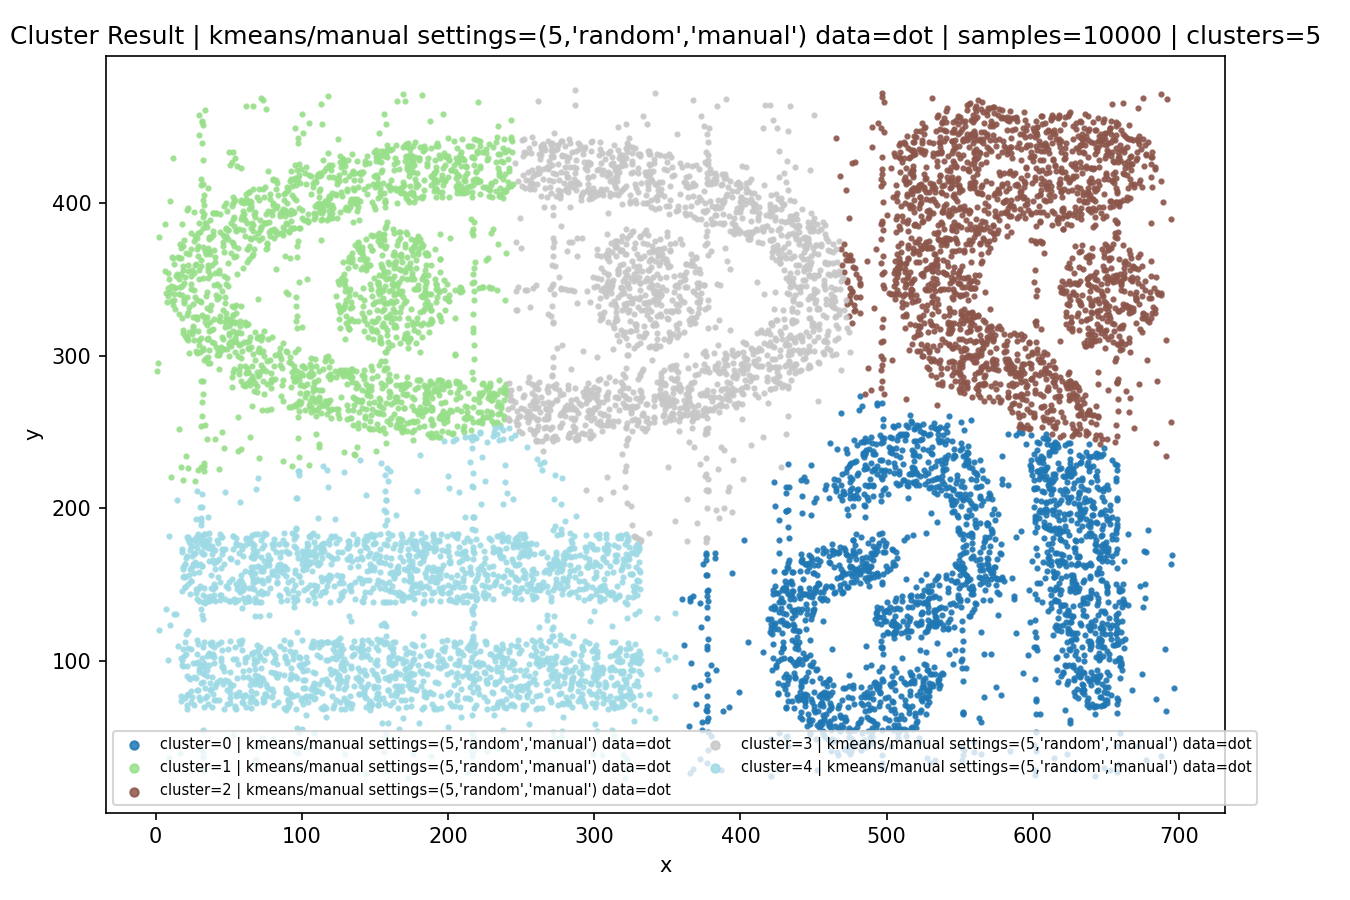
\includegraphics[width=0.48\textwidth]{images/kmeans_manual_clusterData1.10k_dot.png}
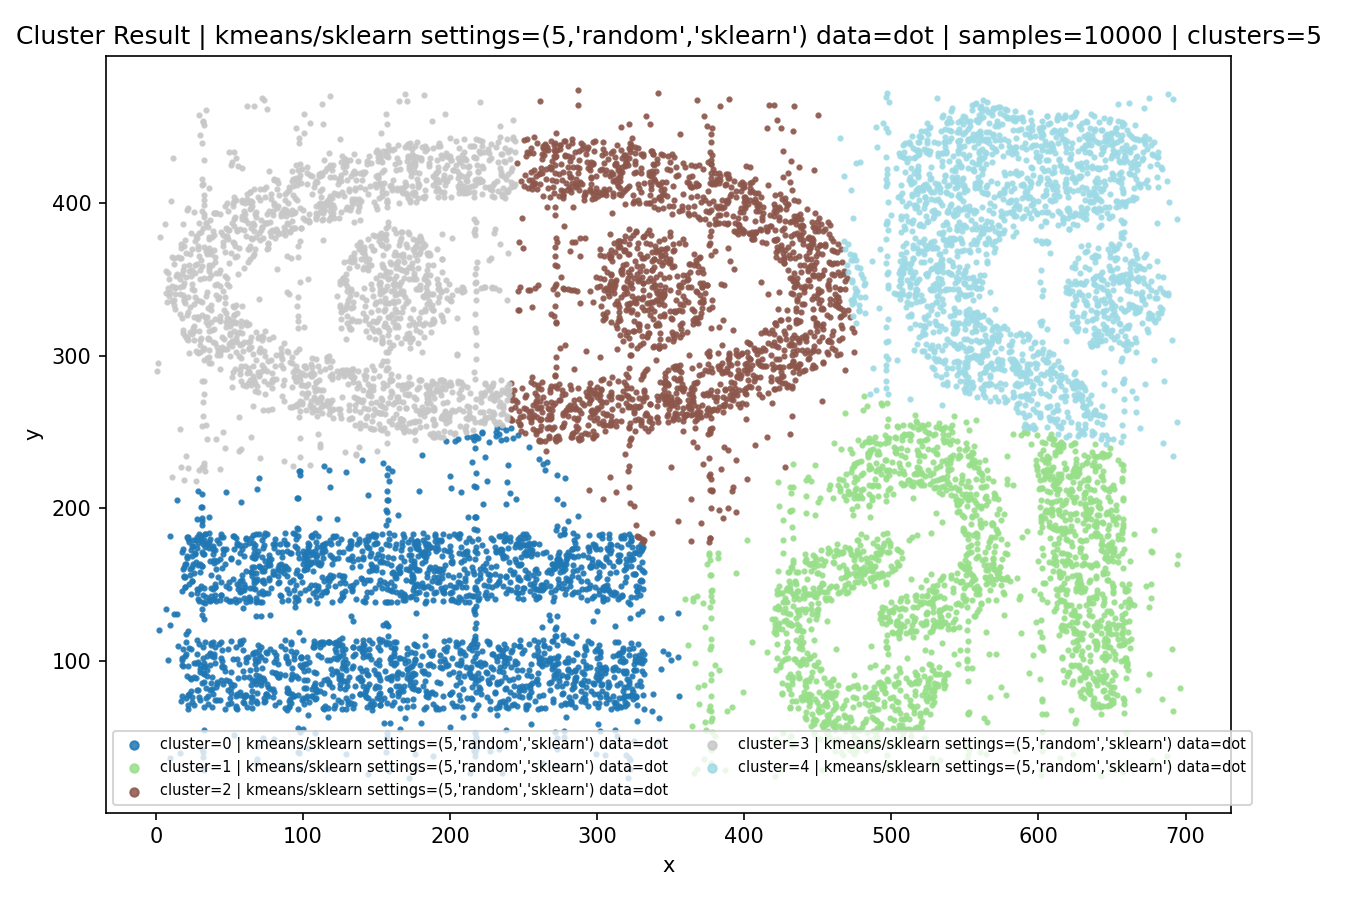
\includegraphics[width=0.48\textwidth]{images/kmeans_sklearn_clusterData1.10k_dot.png}
\caption{二维点数据上的 KMeans 结果对比（左：手写版，右：sklearn 版）}
\label{fig:kmeans_dot}
\end{figure}

\begin{figure}[H]
\centering
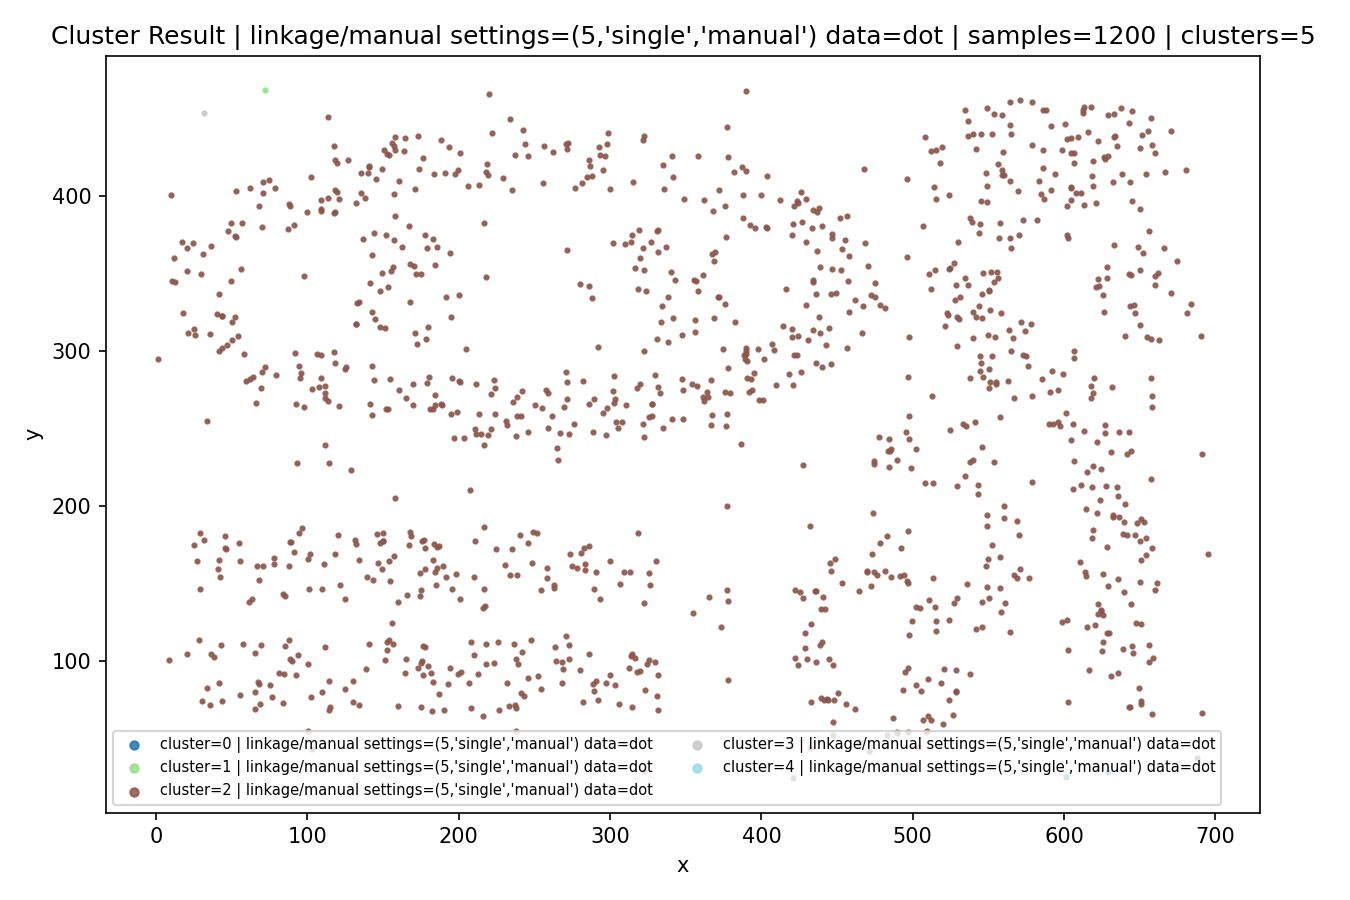
\includegraphics[width=0.48\textwidth]{images/linkage_manual_clusterData1.10k_dot.png}
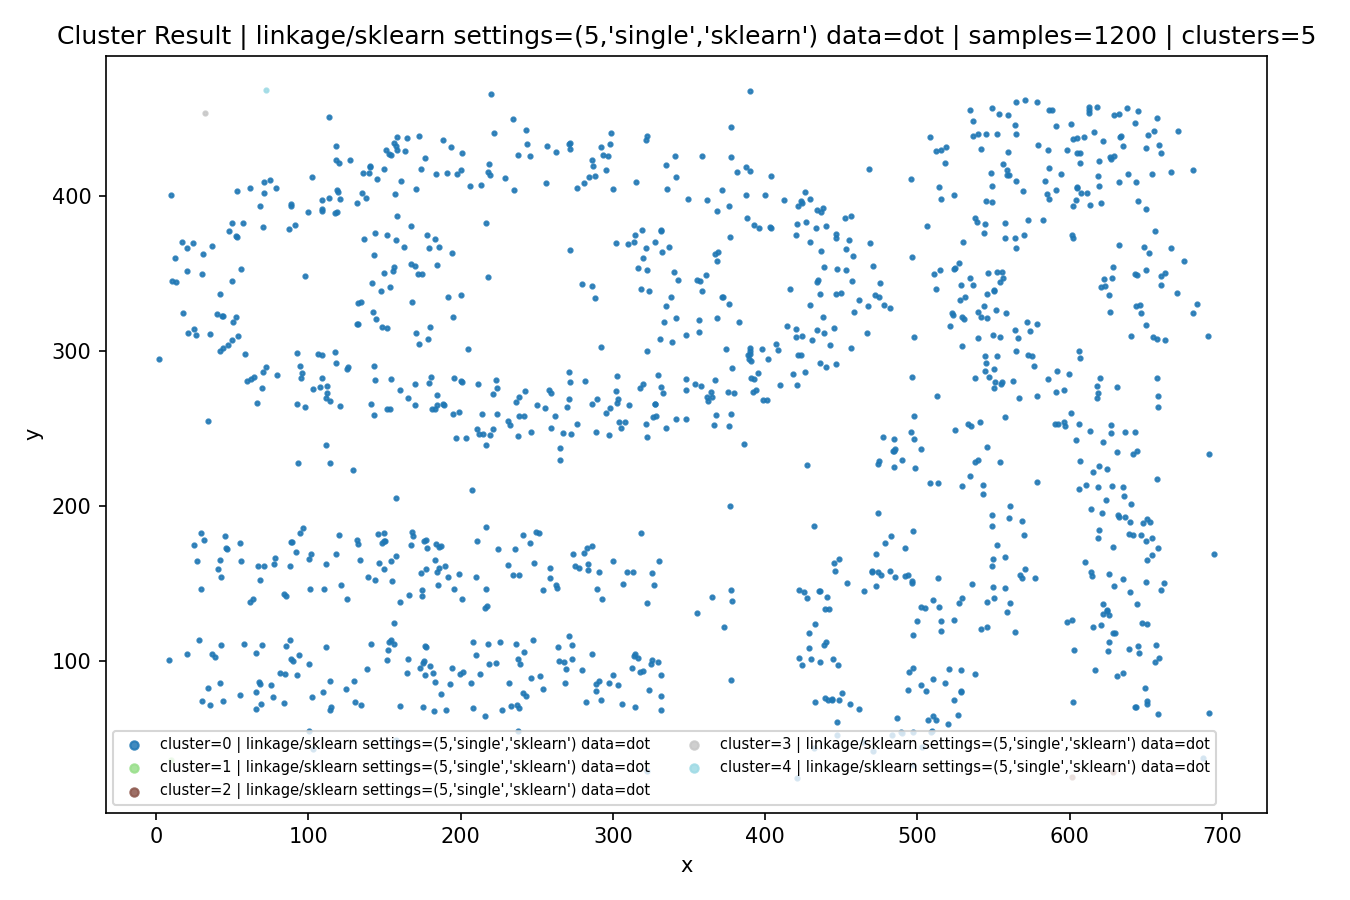
\includegraphics[width=0.48\textwidth]{images/linkage_sklearn_clusterData1.10k_dot.png}
\caption{二维点数据上的层次聚类结果对比（左：手写版，右：sklearn 版）}
\label{fig:linkage_dot}
\end{figure}

\begin{figure}[H]
\centering
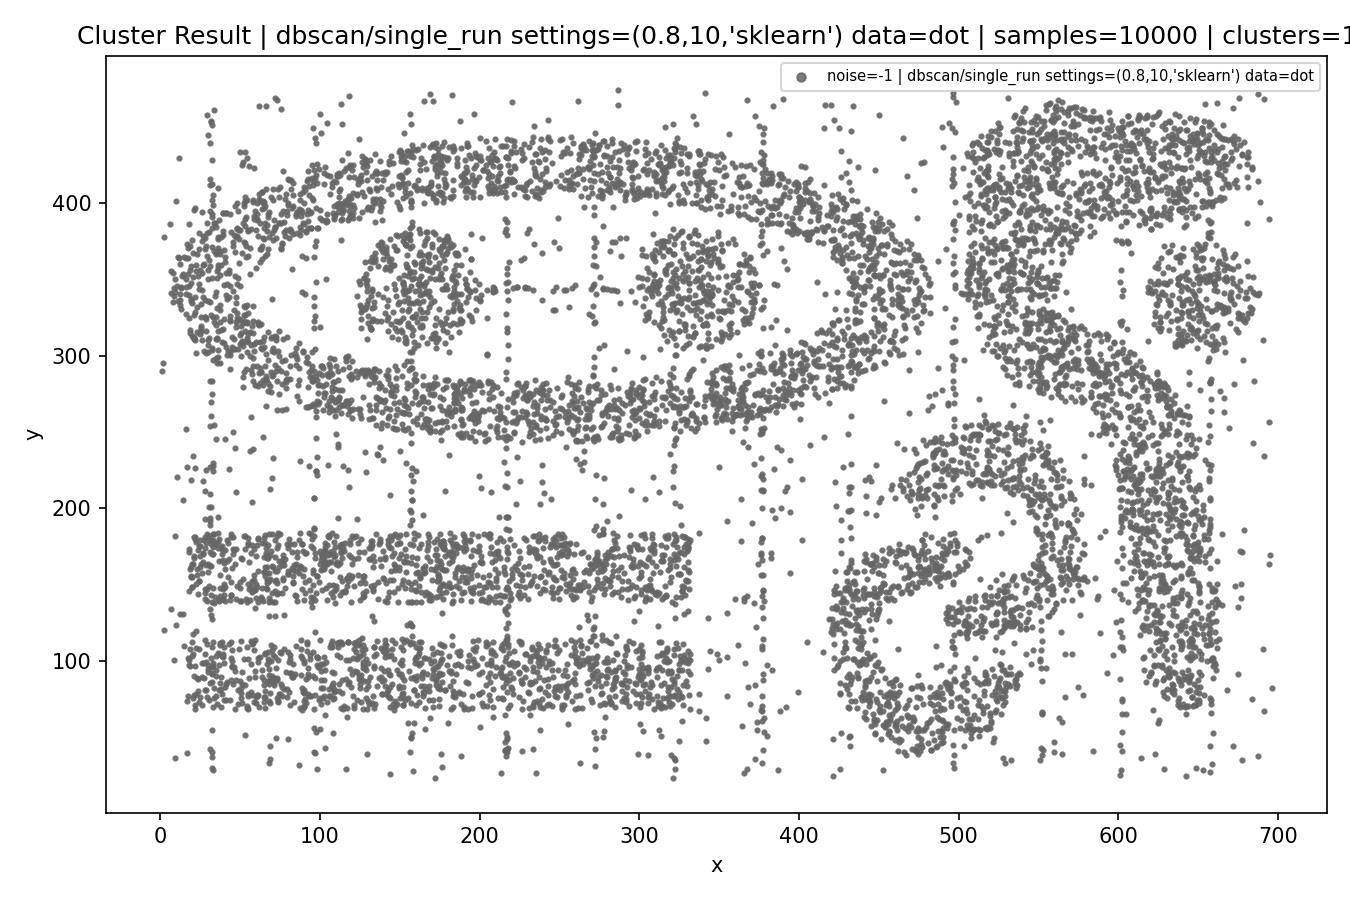
\includegraphics[width=0.8\textwidth]{images/dbscan_single_run_clusterData1.10k_dot.png}
\caption{二维点数据上的 DBSCAN 结果}
\label{fig:dbscan_dot}
\end{figure}

结果分析：
\begin{itemize}
  \item KMeans 的手写版和 sklearn 版图形几乎一致，说明手写实现与标准实现基本等价。
  \item KMeans 对这类弯曲、细长结构的拟合能力有限，因此能分出若干区域，但不能完整恢复所有非凸形状。
  \item single-link 层次聚类容易发生“链式合并”，一些相邻但语义上不同的区域会被连成一个大簇。
  \item DBSCAN 的这组参数偏严格，图中噪声点较多，说明 \texttt{eps} 对当前数据尺度过小，参数需要重新调整。
\end{itemize}

\subsection{任务二结果：时序数据聚类指标}
时序数据的实验结果如下。

\begin{table}[H]
\centering
\caption{时序数据聚类结果}
\label{tab:timeseries}
\begin{tabular}{lcccc}
\toprule
算法 & 实现 & ARI & NMI & 运行时间(s) \\
\midrule
KMeans & manual & 0.3360 & 0.5117 & 0.0009 \\
KMeans & sklearn & 0.3341 & 0.5104 & 0.0550 \\
linkage & manual & 0.0019 & 0.0870 & 0.0194 \\
linkage & sklearn & 0.0019 & 0.0870 & 0.0225 \\
DBSCAN & sklearn & 0.0032 & 0.0408 & 0.0018 \\
\bottomrule
\end{tabular}
\end{table}

结果分析：
\begin{itemize}
  \item KMeans 在该数据上效果最好，ARI 和 NMI 都明显高于另外两种方法，说明特征空间中存在一定的中心型结构。
  \item 手写 KMeans 与 sklearn KMeans 的指标几乎一致，说明实现正确。
  \item 层次聚类和 DBSCAN 的效果较弱，说明这些数据在当前特征表示下并不适合直接用单链合并或密度阈值划分。
\end{itemize}

\subsection{任务三结果：UCI 数据聚类指标}
UCI wine 数据上的结果如下。

\begin{table}[H]
\centering
\caption{UCI wine 数据聚类结果}
\label{tab:uci}
\begin{tabular}{lcccc}
\toprule
算法 & 实现 & ARI & NMI & 运行时间(s) \\
\midrule
KMeans & manual & 0.0342 & 0.0564 & 0.0451 \\
KMeans & sklearn & 0.0325 & 0.0536 & 0.2207 \\
linkage & manual & 0.0001 & 0.0099 & 2.4243 \\
linkage & sklearn & 0.0001 & 0.0099 & 0.0325 \\
DBSCAN & sklearn & -0.0010 & 0.0466 & 0.1295 \\
\bottomrule
\end{tabular}
\end{table}

结果分析：
\begin{itemize}
  \item 三种算法在 wine 数据上的指标整体较低，说明原始质量标签与无监督聚类结构并不完全一致。
  \item KMeans 虽然比另外两种方法稍好，但提升幅度有限，表明该数据集更适合监督学习或更有针对性的特征工程。
  \item 手写层次聚类在 1200 条采样数据上耗时明显更高，说明单链层次聚类对样本规模较敏感。
\end{itemize}

\section{总结}
本实验完成了聚类算法的实现、对照与分析：
\begin{itemize}
  \item 在原有工程基础上补充了手写 KMeans、手写 SLINK、特征处理、统一结果输出和评估流程。
  \item 在二维点、时序数据和 UCI 数据上比较了 KMeans、层次聚类与 DBSCAN 的适应性。
  \item 结果表明：KMeans 更适合紧凑型簇，single-link 易链式合并，DBSCAN 对参数和尺度最敏感。
\end{itemize}

本次实验也说明，聚类算法的表现不仅取决于算法本身，还强烈依赖于数据表示、参数选择和评价方式。对于复杂数据，先做合适的特征工程和参数搜索往往比直接套用算法更重要。

\section*{附录：实验源代码与运行命令}
\subsection*{A.1 主要改动文件}
\begin{itemize}
  \item \texttt{clustering.py}：数据读取、实验入口、评估与图片输出。
  \item \texttt{kmeans.py}：手写 KMeans 与 sklearn 对照。
  \item \texttt{linkage.py}：手写 single-link（SLINK）与 sklearn 对照。
  \item \texttt{features.py}：点数据与时序数据特征处理。
\end{itemize}

\subsection*{A.2 关键代码片段}
\begin{lstlisting}
# clustering.py 中统一把输出保存到 results/ 目录
RESULT_DIR = "results"

def ensure_result_dir():
    os.makedirs(RESULT_DIR, exist_ok=True)

# 对二维点数据输出带有算法和参数说明的图像
output_name = "%s_%s_%s_%s.png" % (model_name, run_name, data_name, data_type)
method_desc = "%s/%s settings=%s data=%s" % (model_name, run_name, safe_settings, data_type)
\end{lstlisting}

\subsection*{A.3 运行命令}
\begin{verbatim}
# 二维点数据：同时比较三种算法
python clustering.py -d dots/clusterData1.10k.dat -t dot -m all

# 时序数据：比较三种算法
python clustering.py -d timeSeries/Plane_TRAIN.txt -t timeseries -m all

# UCI 数据：比较三种算法
python clustering.py -d wine+quality -t uci -m all

# 参数扫描
python clustering.py -d wine+quality -t uci -m all --sweep
\end{verbatim}

\end{document}
